\chapter{使用工作區}\label{ch:workspace}
\chapterlead{工作區既是觀察結構的地方，也是組織計算和儲存結果的地方。本章從主視窗的各個區域入手，透過匯入、檢視、命名和儲存一個矽結構專案，建立後續教程共同使用的操作習慣。}

\section{主視窗的佈局}
\index{Gongzuoqu@工作區}
工作區把結構、計算步驟和結果放在同一個主視窗中。先認識初次進入時的空白布局，再展開練習中需要的面板，就容易分清“專案中有什麼”和“當前正在編輯什麼”。頂部功能區用於選擇命令，中央文件區用於顯示結構、工作流與圖形；兩側面板提供專案條目、物件資訊、計算引數和執行輸出。

\subsection{初次進入工作區}
第一次進入空白專案時，中央顯示歡迎文字，還沒有開啟結構或工作流文件。圖\ref{fig:desktop-start}展示這一佈局：左側專案瀏覽器列出專案分類，資訊瀏覽器位於左下方並摺疊為標題欄，右側面板組尚未展開。空白文件區是開始工作的地方；匯入結構或建立工作流後，相應文件才會出現在這裡。

\begin{figure}[!htb]
\centering
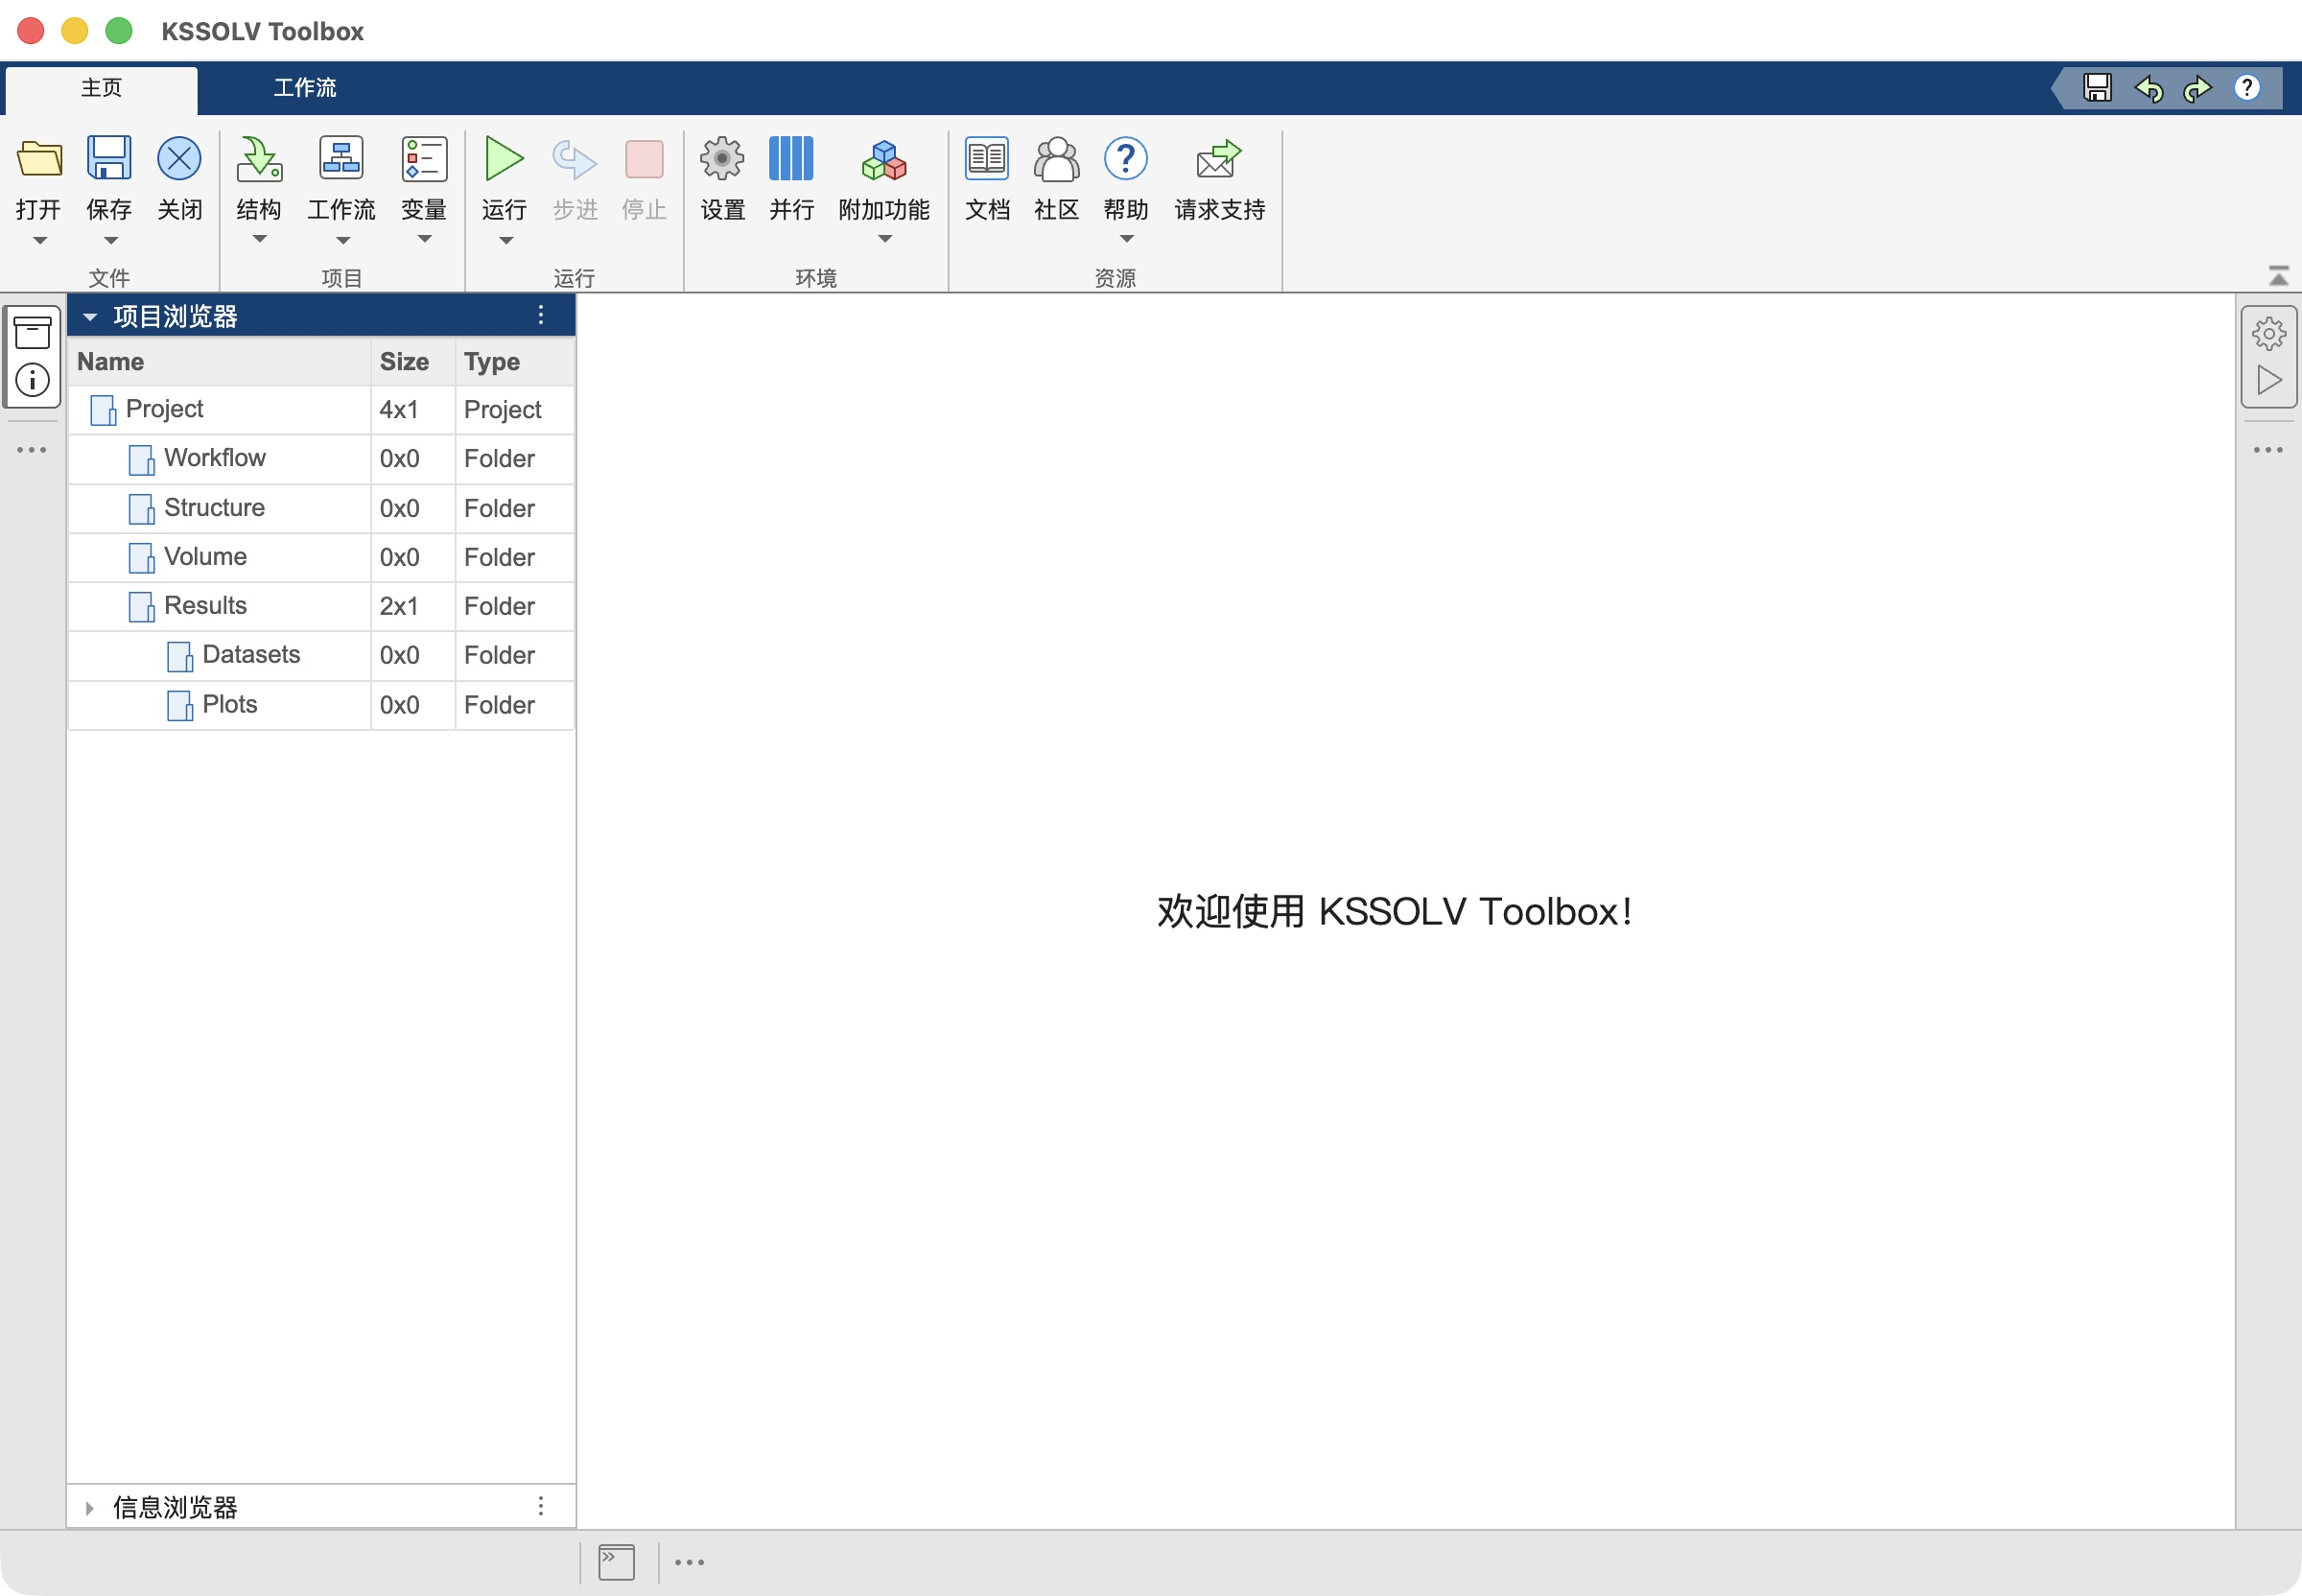
\includegraphics[width=\linewidth]{publication-assets/crop-eb25a0cdb09d3f78fdbd.png}
\caption{獨立應用程式的初始工作區。中央尚未開啟文件，左側專案瀏覽器列出專案分類；資訊瀏覽器摺疊為標題欄，右側面板組處於收起狀態。}
\label{fig:desktop-start}
\end{figure}

可以先找到\ui{主頁}中的\ui{結構}與\ui{工作流}入口，再觀察視窗兩側的按鈕。左側的專案與資訊圖示控制同一組面板，右側的配置與執行圖示控制另一組面板；點選按鈕組可以收起或展開這一側的區域。組內面板標題前的小三角用於單獨展開內容。需要的面板沒有出現時，從側邊欄省略號開啟\ui{開啟面板}列表，按名稱選擇即可。

\subsection{展開練習需要的面板}
做第一次計算時，通常需要在專案、結構、工作流和引數之間來回檢視。圖\ref{fig:install-workspace-overview}展示空專案中展開主要面板後的佈局：左側顯示專案與資訊，右側顯示配置與模擬，下方開啟命令列視窗，中央顯示歡迎文字。首次啟動時，部分面板處於收起狀態。

可以依次展開左右面板組，開啟各面板的內容，先熟悉它們的位置。匯入結構或建立工作流後，專案樹才會增加相應條目，中央也會出現文件標籤。雙擊專案條目可以開啟文件，再用標籤選擇當前活動文件：檢視結構時，中央顯示三維模型；切換到工作流標籤時，中央顯示節點和連線。準備配置節點或執行計算前，先核對活動標籤中的工作流名稱。



\begin{table}[!htb]
\centering
\caption{工作區的主要區域與第一次檢視時的操作。}
\label{tab:workspace-regions}
\begin{tabularx}{\linewidth}{p{24mm}p{32mm}X}
\toprule
區域 & 在哪裡 & 先做什麼 \\
\midrule
功能區 & 視窗上方 & 在\ui{主頁}找到結構匯入、工作流、儲存和執行入口。 \\
快捷工具條 & 視窗右上方 & 辨認儲存、撤銷、重做和幫助按鈕。 \\
專案與資訊面板 & 左側按鈕組內 & 辨認專案分類；匯入結構後選擇條目，檢視它的資訊。 \\
配置與模擬面板 & 右側按鈕組內 & 找到引數與輸出區域；建立工作流後，再選擇節點進行配置。 \\
文件區 & 視窗中央 & 空專案顯示歡迎文字；開啟文件後，用標籤切換結構或工作流。 \\
命令列視窗 & 展開後的下方區域 & 需要互動命令時再使用；圖形教程可先保留此面板或摺疊它。 \\
分隔線與狀態列 & 面板邊界及視窗底部 & 拖動分隔線調整空間；執行操作時留意底部狀態文字。 \\
\bottomrule
\end{tabularx}
\end{table}

佈局可以隨任務調整。觀察三維結構時，收起暫時不用的側面板；填寫計算引數時，給配置編輯器更多寬度。拖動面板邊界可以改變左右寬度或上下比例，結構和工作流仍保留在專案中。後面各小節分別說明這些區域怎樣使用；本章的矽晶體練習會從匯入結構開始，逐步用到它們。

\subsection{功能區}
\ui{主頁}包含檔案、專案、執行、環境和資源等常用操作。\ui{開啟}讀取已有專案；\ui{儲存}把當前工作寫入專案檔案；\ui{結構}選單用於新建或匯入結構；\ui{工作流}選單提供建立、模板、匯入與匯出入口。執行計算時使用\ui{執行}，應用設定和幫助也從主頁進入。

\ui{工作流}頁面提供節點與畫布操作。它與中央的工作流文件配合使用：先啟用目標工作流，再新增、連線和配置節點。只有頂部切換到工作流頁面，還不足以確定要執行哪個工作流，應同時檢視中央文件標籤。

當三維結構文件處於活動狀態時，功能區會出現\ui{晶體建模}或\ui{分子建模}頁面。它們是圍繞當前文件提供的工具。切換到其他型別文件後，上下文頁面可能隨之變化。需要建模命令卻看不到相應頁面時，先回到結構標籤，而不是重新匯入結構。

\subsection{專案瀏覽器}
\index{Xiangmu liulanqi@專案瀏覽器}
專案瀏覽器以樹形方式顯示內容，主要分支為 \ui{Workflow}、\ui{Structure}、\ui{Volume} 和 \ui{Results}。結果下又可見 \ui{Datasets} 和 \ui{Plots}。這裡的英文名稱與介面一致，分別表示工作流、原子結構、體資料、數值資料和圖形。

單擊條目用於選擇，雙擊可以開啟相應文件。展開分支後，可同時保留多個專案項；關閉中央文件標籤，只是結束這一個檢視，不等於從專案中刪除它。再次在樹中雙擊，便可重新開啟。選擇刪除操作則會改變專案內容，二者應分清。

樹中的 \ui{Name} 是顯示名稱，\ui{Type} 表示物件型別。\ui{Size} 是專案項組織或資料尺寸資訊，不宜直接當作體系原子數。判斷一個晶體含多少獨立原子，應檢視結構資訊或三維檢視中的位點數。螢幕還可能顯示相鄰晶胞的映像，因此肉眼數到的球體也未必等於模型位點數。

\subsection{資訊瀏覽器}
資訊瀏覽器隨專案瀏覽器的選擇變化。選擇一個結構時，可檢視與該結構有關的屬性；選擇工作流、資料或圖形時，面板顯示對應物件的資訊。它可以幫助確認當前處理的是哪一個條目，避免在相似檔名之間混淆。

部分條目允許編輯顯示名稱。修改後，應在專案樹與文件標籤中核對新名稱。為結構命名時，寫出材料和主要變化通常比 \file{Structure1} 更有用，例如 \file{Si-primitive}、\file{Si-2x2x2}、\file{Si-vacancy}。晶胞和原子數可在結構資訊中檢視。

\subsection{配置編輯器}
\index{Peizhi bianjiqi@配置編輯器}
配置編輯器用於修改工作流節點的引數。先在畫布中選中節點，再點選\ui{工作流 → 配置節點}，或使用節點上的齒輪按鈕。隨後在右側編輯器中向下檢視該節點的\ui{選項}。節點名稱、輸入和輸出等通用欄位，與截斷能、迭代次數等任務引數位於不同區域；只看到通用欄位時，應先執行配置節點命令，再滾動檢視選項。填寫後切換到其他節點，再返回確認數值仍在，是檢查輸入是否提交的簡便方法。

\subsection{檢視執行輸出}

\ui{模擬瀏覽器}顯示執行輸出。自洽場迭代、計算訊息和錯誤資訊往往從這裡開始閱讀。計算結束後，檢視輸出末尾的結束訊息，以及專案結果分支中新生成的資料。第\ref{ch:first}章將用一次小型計算說明如何判斷完成狀態。

\subsection{安排面板佈局}
\index{Cebianlan@側邊欄}
文件區可以同時開啟結構、工作流和圖形標籤。選擇標籤會改變當前活動文件。標籤暫未顯示時，將滑鼠移到文件區上方，可檢視文件標題與標籤。執行工作流前，尤其要看清活動的工作流名稱。多個相似任務並存時，給它們清楚命名，可以減少誤執行。

主視窗兩側設有側邊欄按鈕組。左側的專案與資訊圖示屬於同一組，右側的配置與執行圖示屬於另一組。按鈕組控制這一側面板區域的收放：例如，收起左側組時，專案瀏覽器與資訊瀏覽器一起隱藏；重新展開後，可以繼續使用這兩個面板。右側組展開後，可以同時檢視配置編輯器與模擬瀏覽器。圖\ref{fig:desktop-start}中的右側組處於收起狀態；圖\ref{fig:install-workspace-overview}則展示手動展開後的佈局。

組內各面板還可以單獨摺疊。初始工作區左下方的\ui{資訊瀏覽器}只顯示標題欄；點選標題前的小三角，可以展開下方的資訊區。需要增加三維檢視空間時，可以摺疊某一面板，也可以收起整個側邊組，二者作用的範圍不同。

側邊欄底部的省略號開啟\ui{開啟面板}列表。找不到某個面板時，按名稱選擇\ui{專案瀏覽器}、\ui{資訊瀏覽器}、\ui{配置編輯器}、\ui{模擬瀏覽器}或\ui{命令列視窗}。圖\ref{fig:panels-gallery}顯示線上版中的同組入口，其中還提供\ui{檔案}，用於管理雲端目錄；前述五個面板在獨立版中也可開啟。

\begin{figure}[!htb]
\centering
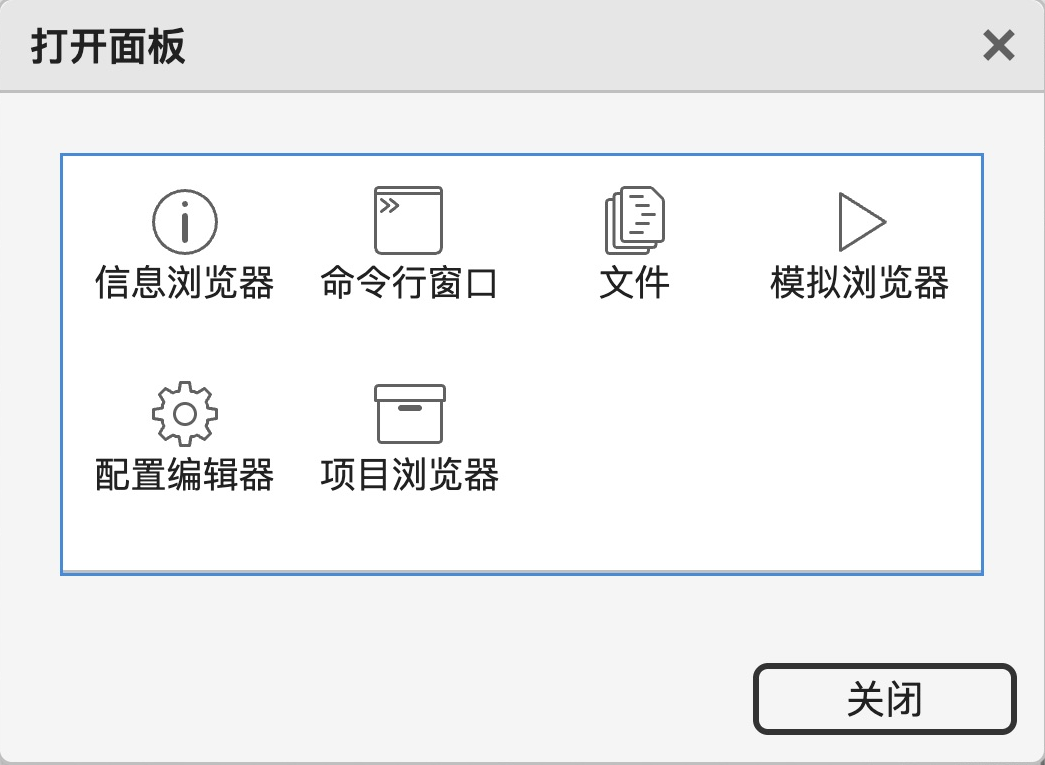
\includegraphics[width=88mm]{publication-assets/crop-50f2208998010f44014c.png}
\caption{面板列表。按名稱開啟具體面板，兩側的按鈕組用於收放成組的面板區域。\ui{檔案}用於管理雲端目錄。}
\label{fig:panels-gallery}
\end{figure}

觀察三維模型時，可以收起暫時不用的引數和輸出面板；編輯引數時，再展開配置編輯器。拖動文件區與面板之間的分隔線，可調整各區域寬度。同組面板之間的分隔線可調整上下比例。可根據螢幕尺寸調整面板寬度。

\section{練習：匯入並檢查矽晶體}
本例使用隨書的 \file{silicon.cif}。它是邊長約 $5.44370\,\text{\AA}$ 的矽常規晶胞，顯式列出 8 個矽位點。檔案採用 P1 方式列出所有位置，便於練習時直接核對原子數。該晶格常數是本例輸入，不是這一步匯入操作計算出的結果。

\begin{figure}[!htb]
\centering
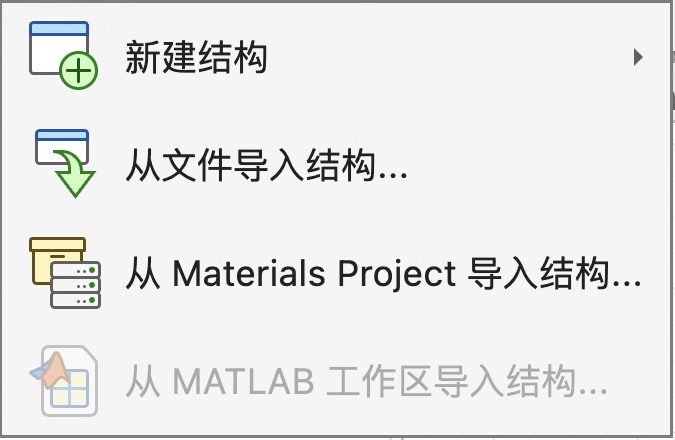
\includegraphics[width=67mm]{publication-assets/crop-e572efea8aa253089edc.png}
\caption{主頁中的結構選單。本練習選擇\ui{從檔案匯入結構}；Materials Project 是另一個結構來源。\ui{從 MATLAB\regmark{} 工作區匯入結構}需要 MATLAB\regmark{} 工具箱環境。}
\label{fig:structure-import-menu}
\end{figure}

\begin{steps}
\item 在\ui{主頁}開啟\ui{結構}選單，選擇\ui{從檔案匯入結構}。
\item 進入隨書示例目錄，選擇 \file{silicon.cif}，確認開啟。
\item 等待專案瀏覽器的 \ui{Structure} 分支出現 \file{silicon}，中央開啟三維結構文件。
\item 拖動檢視旋轉，使用滾輪縮放。使整個晶胞位於畫面中，不必立即調整所有顯示引數。
\item 檢查元素為 Si，模型獨立位點為 8。若看到更多球體，檢視它們是否屬於邊界或相鄰晶胞的顯示映像。
\item 單擊一個位點，檢視原子資訊；使用空白處或相應選擇命令清除選擇，再觀察完整結構。
\end{steps}

\begin{figure}[!htb]
\centering
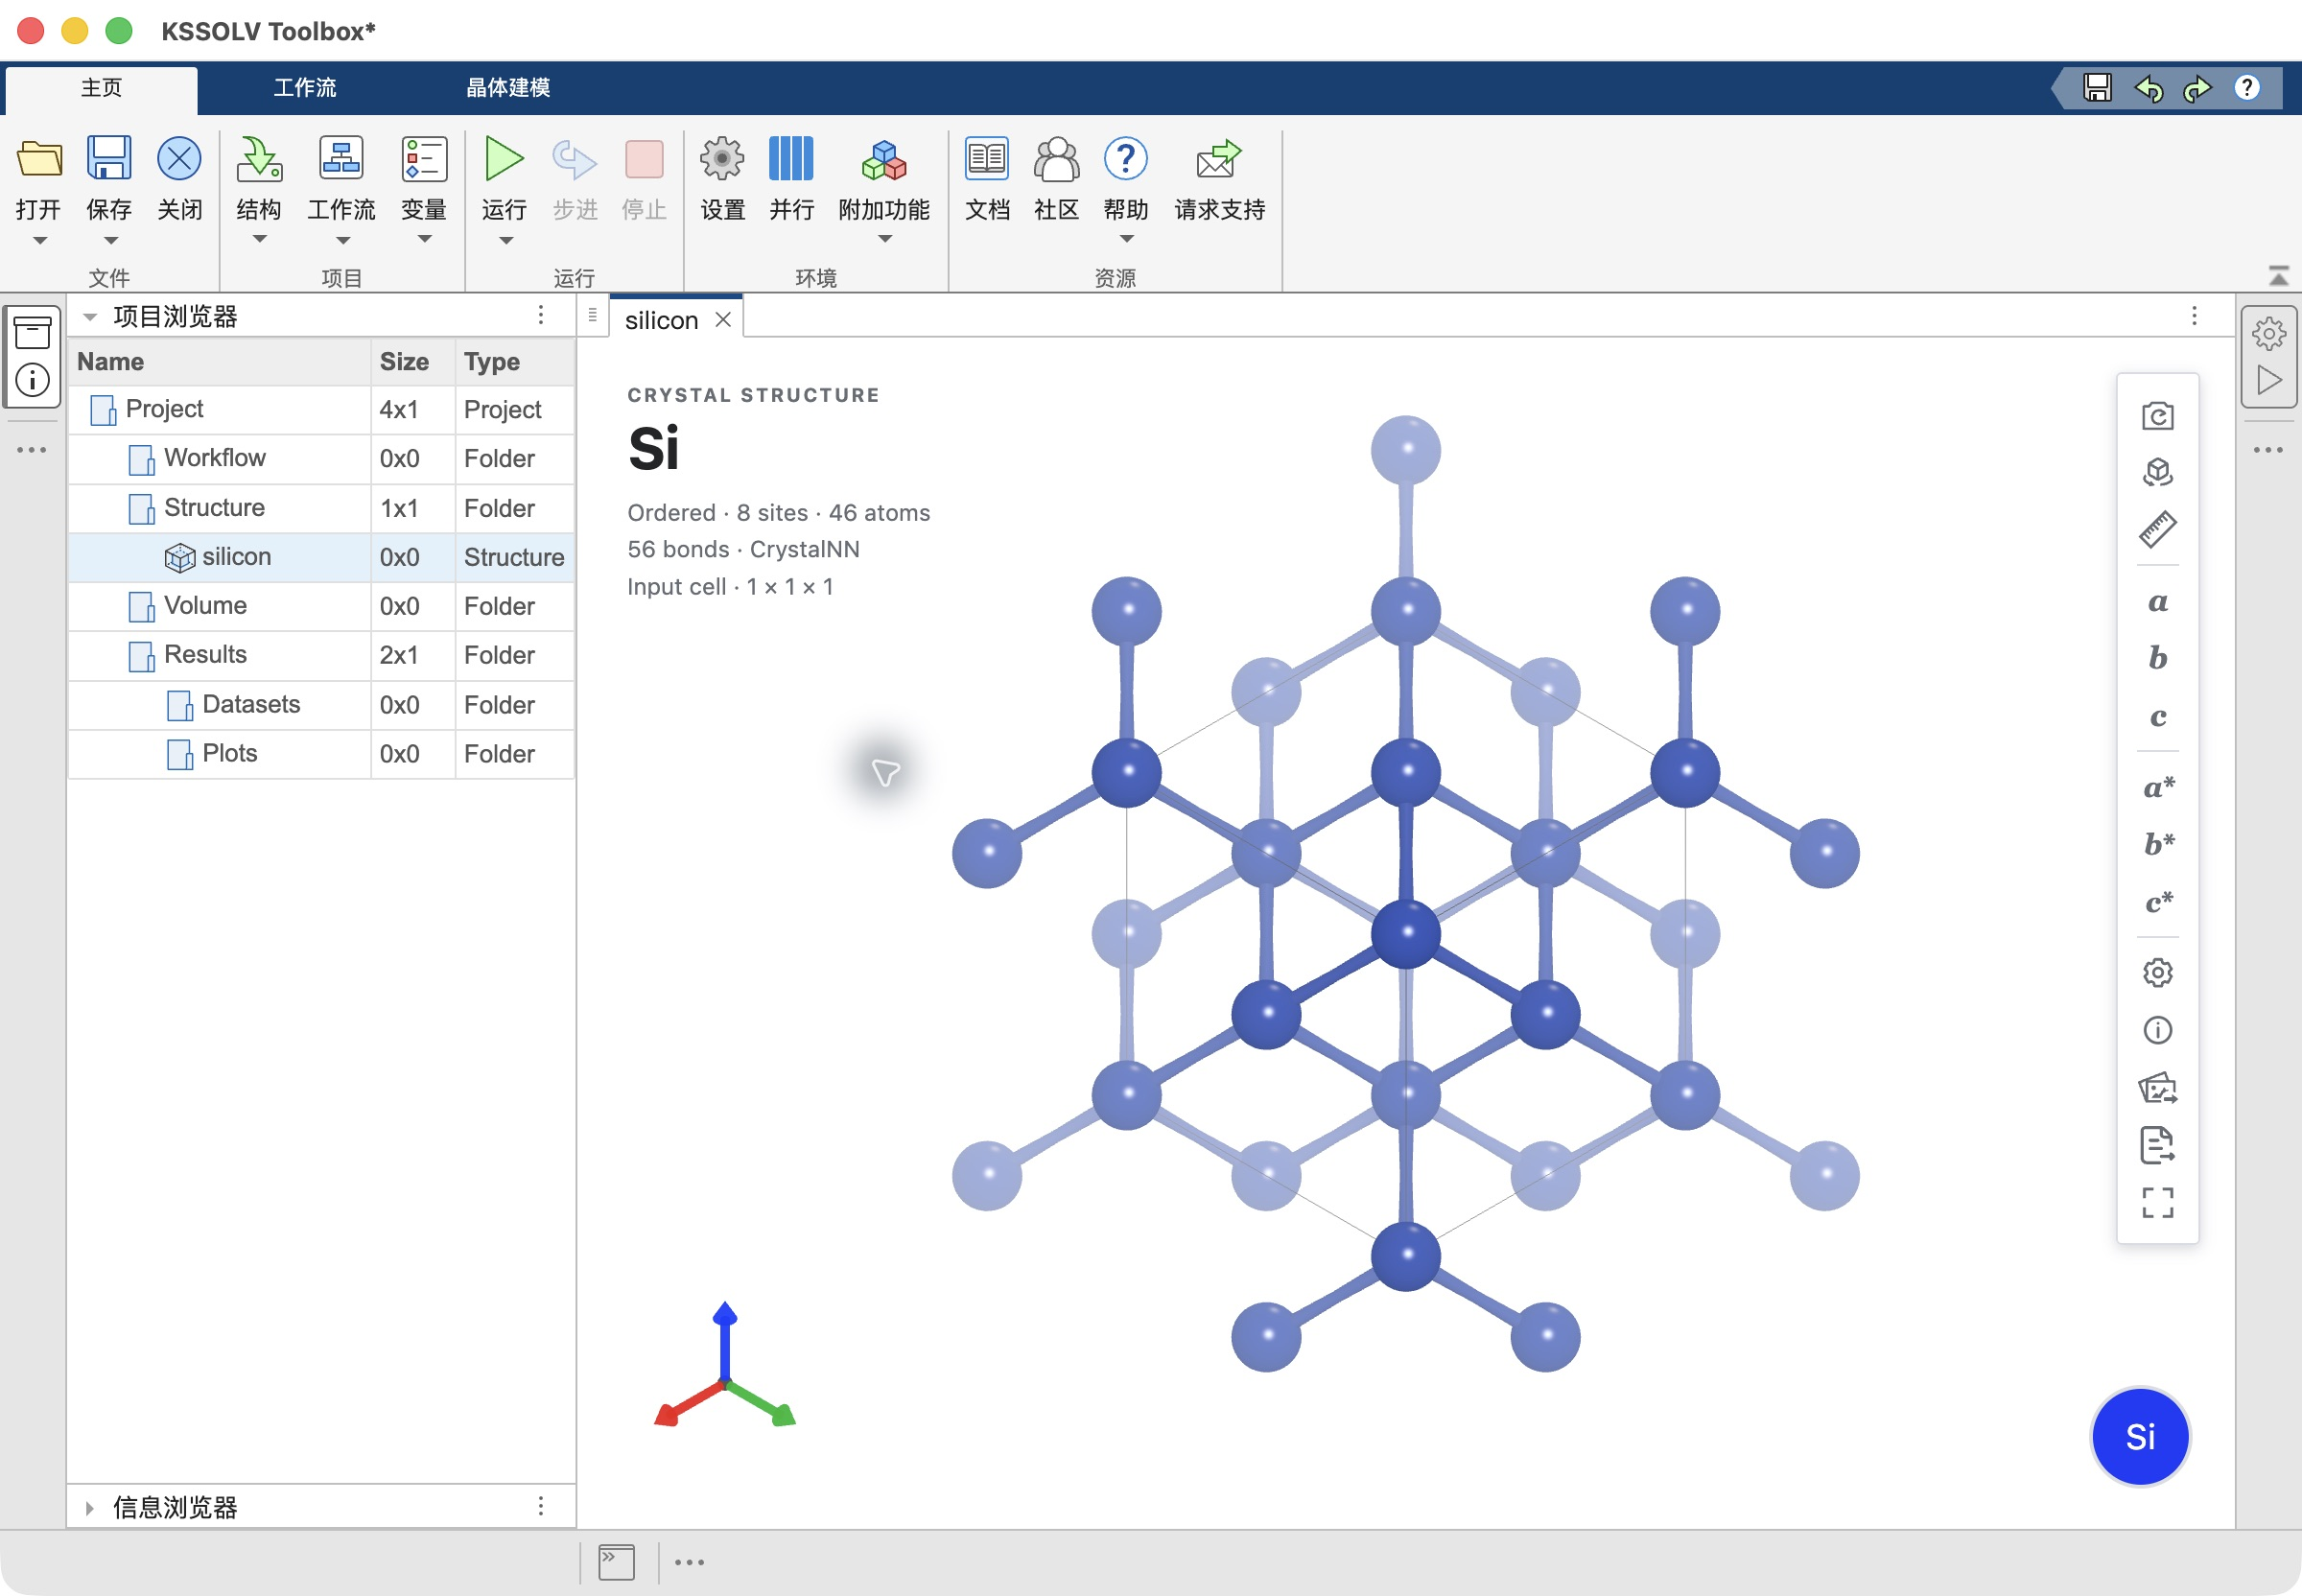
\includegraphics[width=\linewidth]{publication-assets/crop-693a9be4f512a9a0e125.png}
\caption{匯入隨書矽晶體後的結構文件。檢視左上方顯示\ui{8 sites · 46 atoms}：輸入模型有 8 個位點，當前三維畫面連同週期邊界映像共繪製 46 個球體。}
\label{fig:silicon-import}
\end{figure}

\subsection{一次匯入多個檔案}

桌面檔案選擇器允許多選結構檔案。需要比較一組模型時，使用\ui{從檔案匯入結構}，在檔案視窗中選中這些輸入後一起開啟；每個成功讀入的檔案會成為獨立的專案結構，而不是把所有原子自動拼成一個模型。

匯入結束後，在Structure分支逐個開啟新增結構進行檢查。若個別檔案無法解析，可按輸出提示單獨處理；已成功匯入的其他結構仍保留在專案中。線上版先將多個檔案上傳到雲端目錄，再按檔案面板的匯入方式逐項加入專案；上傳成功本身不等於已經匯入。


\subsection{讀懂位點資訊}
檢視左上方概括當前結構和顯示狀態。本例的\ui{8 sites}對應檔案列出的 8 個矽位點；\ui{46 atoms}表示當前畫面中繪製的原子，包括週期邊界附近的映像。下方的\ui{Input cell · 1 × 1 × 1}說明正在按輸入晶胞顯示。邊界處顯示更多球體，有助於看清跨晶胞的連線關係，並不表示輸入已擴成含 46 個獨立原子的模型。

在三維檢視中選擇一條矽—矽鍵，可以檢視它連線的位點與幾何長度。圖\ref{fig:silicon-bond-inspection}的檢查卡片顯示\ui{Sites 2–7}，鍵長為 $2.35719\,\text{\AA}$，週期映像編號為\ui{0, 0, 0}。其中，位點編號用於對應模型中的原子；映像編號表示這條連線所用的晶胞平移。檢查其他連線時，應同時看這兩項。

\begin{figure}[!htb]
\centering
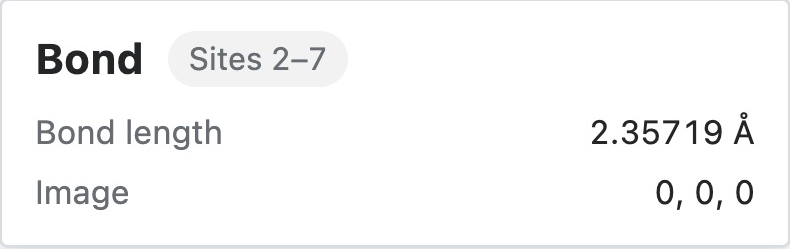
\includegraphics[width=79mm]{publication-assets/crop-6bd0b3f7b04c691f91a8.png}
\caption{選擇矽—矽鍵後的檢查卡區域性。卡片中的 $2.35719\,\text{\AA}$ 為輸入結構中這條鍵的幾何長度。}
\label{fig:silicon-bond-inspection}
\end{figure}

完成檢查後，清除選擇，恢復完整檢視。當前步驟的目的，是確認檔案、模型位點和顯示映像之間的對應關係。後續進行擴胞或結構最佳化時，也沿用這一檢查方法：先讀結構資訊，再檢查所關心的原子與連線。

若讀取的是其他來源 CIF，匯入後應先核對晶胞、佔位、元素及原子數。不同檔案可能使用原胞、常規晶胞或部分佔位，不能僅憑化學式相同就假定結構相同。先把檔案本身的描述認清，再決定是否轉換或擴胞。

\section{儲存專案}
\index{Baocun xiangmu@儲存專案}
\subsection{首次儲存}
\begin{steps}
\item 在\ui{主頁}點選\ui{儲存}。
\item 獨立版選擇自己的工作目錄，輸入 \file{Si-introduction.ks}。線上版按第\ref{ch:online}章的方法選擇雲端目錄。
\item 確認儲存後，檢視視窗標題和專案檔名。
\item 再做一個容易識別的小改動，例如更改結構的顯示名稱，觀察標題中的星號。
\item 再次儲存，確認專案寫入完成。
\end{steps}

標題中的星號表示尚有修改。儲存既用於保留工作流和結果，也會處理結構編輯中的待儲存內容。建模有預覽、應用與儲存幾個階段：預覽用來檢查，應用確認這一次修改，儲存才把當前工作寫入專案檔案。第\ref{ch:modeling}章會透過實際編輯說明這些階段。

\subsection{為不同研究保留副本}
當一個專案將用於多個不同條件時，可使用\ui{另存為}建立分支。例如，先儲存原始矽專案，再另存成 \file{Si-supercell.ks} 做擴胞。這樣能夠保留清楚的起點。只更改專案名稱不會自動改變模型，仍應在結構資訊中確認是否已執行所需操作。

對同一個體系比較不同截斷能時，也可在專案中保留多個明確命名的工作流。若結果較多或差異很大，分成多個專案更容易整理。選擇哪種方式取決於工作習慣，關鍵是能從結果追溯到所用結構和引數。

\subsection{重新開啟檢查}
完成本例後，可關閉當前專案，再用\ui{開啟}讀取剛儲存的 \file{.ks} 檔案。展開結構分支，雙擊矽結構，檢查它能重新顯示。這個小練習確認儲存的是可繼續工作的專案，而不僅是當前螢幕上的一張圖。

線上版中，重新開啟雲端專案與開啟本機下載副本是兩種入口。前者在檔案面板選擇已有 \file{.ks}；後者先上傳本機副本。專案內容可以相同，存放位置仍需自己確認。

\subsection{關閉當前專案}

\ui{主頁 → 關閉}關閉的是當前整份專案，不只是中央的一張結構標籤。存在未儲存的專案或結構編輯時，會詢問儲存、不儲存或取消。希望繼續留在原專案就選擇\ui{取消}；選擇儲存後，應等待儲存完成再進入空專案。關閉中央文件標籤則保留專案樹中的條目，需要時仍可再次開啟。

\subsection{移除試算條目}

不再需要的工作流、結構或圖形可以從專案中移除。選擇不再使用的條目後執行移除；需要保留某一階段時，可以先另存專案副本。

\begin{steps}
\item 在專案瀏覽器中單擊一條試算記錄，確認選擇的是具體專案項，而不是Project或分類資料夾。
\item 讓焦點留在專案樹，按Backspace移除該項。刪除當前工作流也可先選中其專案條目，再使用工作流頁面的\ui{刪除}。
\item 如果相應文件有未儲存修改，按彈出的關閉提示選擇；取消關閉時應回到專案樹重新核對。
\item 檢查留下的結構和流程仍然對應，再儲存專案。刪除專案項不等於刪除最初從磁碟匯入的原始檔。
\end{steps}


\section{選擇要儲存的檔案}
\index{Xiangmu wenjian@專案檔案}
\file{.ks} 儲存專案整體；\file{.wf} 儲存工作流；CIF、POSCAR、XYZ 等檔案主要儲存結構。分享專案或練習結果時，應根據對方需要選擇檔案。希望對方接著計算，通常提供專案更方便；希望對方使用相同的任務組織方式，但更換材料，可以提供工作流模板；只交換幾何結構，則匯出相應結構檔案。

結構檔案能表達的內容與格式有關。CIF 適合晶胞和晶體位置，XYZ 直觀地表達元素與笛卡爾座標，但普通 XYZ 並不完整描述週期晶胞和顯式化學鍵。儲存重要的分子連線或複雜週期模型時，應檢視所選格式能保留哪些內容，並在重新匯入後檢查。

\section{使用命令列視窗}
\index{Minglinghang@命令列視窗}
命令列視窗為需要互動命令的讀者提供補充入口。獨立應用和線上版中可使用發行包提供的函式與可用內建運算；本書的復算指令碼在完整 MATLAB\regmark{} 中執行。常規匯入、建模和工作流教程不要求使用命令列視窗。使用已有命令時，應先確認命令與當前工作區的物件對應，執行後再回到專案樹或檢視檢查結果。

主頁的\ui{文件}和\ui{幫助}提供進一步閱讀；\ui{幫助 → 關於 KSSOLV}顯示版本資訊。遇到操作與書中不同時，先確認軟體版本和當前文件型別；問題說明與日誌整理見第~\ref{ch:troubleshooting}~章。

\subsection{執行一條簡單命令}

從\ui{開啟面板}列表開啟\ui{命令列視窗}，將游標放在 \texttt{>>} 後的輸入區。輸入一條命令後按 Enter，輸出會接在下方。下面的練習只使用簡單陣列，不改變專案結構。

\Needspace{5\baselineskip}
\begin{lstlisting}[language=Matlab]
a = [1 2 3];
sum(a)
\end{lstlisting}

逐行提交後，第二行應得到 6。輸入\texttt{whos}可以檢視當前命令工作空間中的變數。鍵盤上、下方向鍵用於回到已輸入的命令；Tab 用於選擇補全建議，Esc 關閉建議。輸入\texttt{clc}清除視窗中的顯示記錄，但不等於刪除變數。清空顯示前，需要保留的命令與輸出可以複製到自己的實驗記錄。

命令視窗的變數與專案樹是兩種儲存方式。建立變數\texttt{a}不會在專案裡自動增加一個結構，儲存專案也不是儲存命令視窗全部臨時變數。希望保留結構、流程和結果時，回到專案樹檢查相應條目；希望重複執行一組命令時，在完整 MATLAB\regmark{} 中整理為指令碼。

\section{使用快捷工具條}

主視窗上方的快捷工具條提供儲存、撤銷、重做和幫助。快捷儲存與\ui{主頁 → 儲存}儲存同一個專案，不是另存當前圖片。視窗中同時開啟多個文件時，先確認正在操作哪一個：結構文件活動時，撤銷與重做針對該結構的建模歷史；工作流文件活動時，針對流程圖編輯。

\begin{steps}
\item 在三維結構中完成一次容易識別的編輯，觀察修改後的狀態。
\item 單擊快捷工具條的\ui{撤銷}，確認模型回到前一步；再單擊\ui{重做}恢復。
\item 確認模型正確後，單擊快捷\ui{儲存}，核對專案的儲存標記。
\end{steps}

完成第~\ref{ch:first}~章、建立第一條工作流後，還可以在畫布中移動一個節點，再用撤銷和重做比較兩類編輯。

儲存檔案、執行計算和撤銷編輯不是同一件事。撤銷並不負責恢復外部檔案或取消已經完成的科學計算；比較兩次計算仍應保留不同結果和明確的引數說明。

\section{從 \headinglatin{Materials Project} 查詢結構}\label{sec:mp-search}
\index{Materials Project@Materials Project!Jiansuo@檢索結構}

資料庫檢索適合在尚無本地結構檔案時尋找計算起點。先按第\ref{ch:remote}章在設定中儲存自己的 Materials Project 訪問金鑰，再選擇\ui{主頁 → 結構 → 從 \mbox{Materials Project} 匯入結構…}。檢索視窗上方是查詢條件，中間是元素週期表，下方是結果表與翻頁按鈕。匯入後，可為選定結構繼續建立計算工作流。

\subsection{選擇檢索方式}

\begin{table}[htbp]
\centering
\caption{Materials Project 的三種檢索方式。}
\begin{tabularx}{\linewidth}{lX}
\toprule
方式 & 適用的查詢問題 \\
\midrule
僅這些元素 & 在週期表選擇元素，結果包含全部所選元素且不含其他元素；例如只選 Si，尋找單質矽。 \\
至少包含這些元素 & 所選元素必須出現，結果還可以有其他元素；例如先選 Fe、O，再檢視含它們的材料。 \\
化學式 / MP ID & 直接輸入化學式或已知材料標識；適合按已知記錄查詢。 \\
\bottomrule
\end{tabularx}
\end{table}

前兩種方式透過週期表選擇元素，頂部元素文字隨選擇更新。按化學式查詢時，切換\ui{化學式 / MP ID}。\ui{清除元素}用於清掉週期表中已有的選擇，便於開始新的元素組合。

\subsection{練習：查詢一個矽結構}

\begin{steps}
\item 選擇\ui{僅這些元素}，清除原有選擇，再在週期表選擇 Si。
\item 單擊\ui{檢索}，等待狀態列結束查詢。若沒有記錄，先確認查詢方式與元素選擇，再檢查訪問設定。
\item 在結果中檢視\ui{Material ID}、化學式、晶系、空間群和原子數。相同化學式可能對應不同結構，不能只憑第一行決定。
\item 每頁條數可選10、15、20或30；用首尾頁與前後頁按鈕繼續檢視。需要比較某列時，可單擊表頭排序當前結果。
\item 本例選擇\ui{mp-149}，其晶系為Cubic、空間群為Fd-3m（227）、原子數為2。選擇這一行，使\ui{匯入所選結構}可用，單擊匯入並等待結構取得完成。
\item 關閉檢索視窗，切回專案瀏覽器，找到新增加的 Structure 條目。開啟三維文件，核對元素、晶胞和獨立位點數，再儲存專案。
\end{steps}

檢索結果隨資料庫更新而變化，查詢時按 Material ID 和結構資訊確認材料。mp-149匯入的是兩位點原胞，與八位點常規矽晶胞是同一晶體的不同晶胞表示。需要與隨書矽數值逐項比較時，仍使用指定的\file{silicon.cif}或\file{silicon_primitive.cif}，保持輸入一致。

結果表還顯示體積、密度、帶隙、形成能、凸包能和穩定性。單位已經寫在列名中：帶隙為 eV，形成能與凸包能為 eV/atom。這些數值來自資料庫，引用時應註明相應記錄。星號表示實驗中已觀測到的記錄。記錄下 Material ID，有助於在報告中說明結構來源。


\begin{figure}[!htb]
\centering
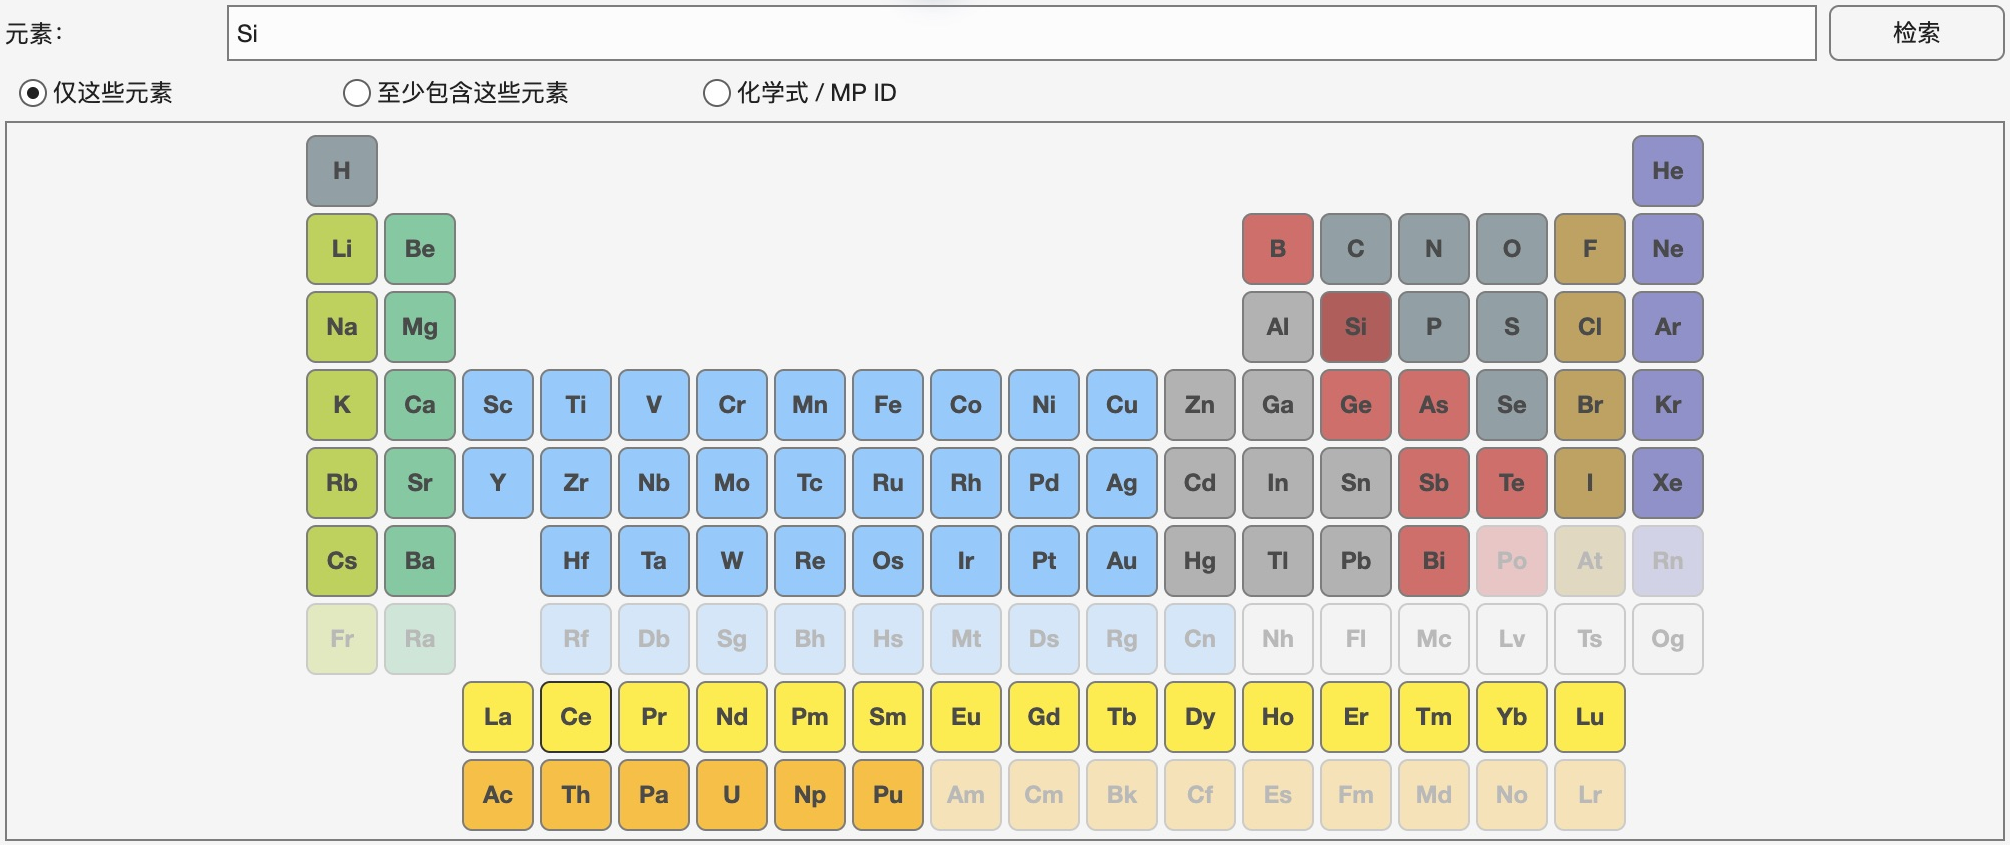
\includegraphics[width=\linewidth]{publication-assets/revision-materials-project-si-results.png}
\caption{在元素週期表選擇Si，使用“僅這些元素”查詢單質矽。查詢方式與元素選擇顯示在結果表上方。}
\label{fig:mp-periodic-live}
\end{figure}

\begin{figure}[!htb]
\centering
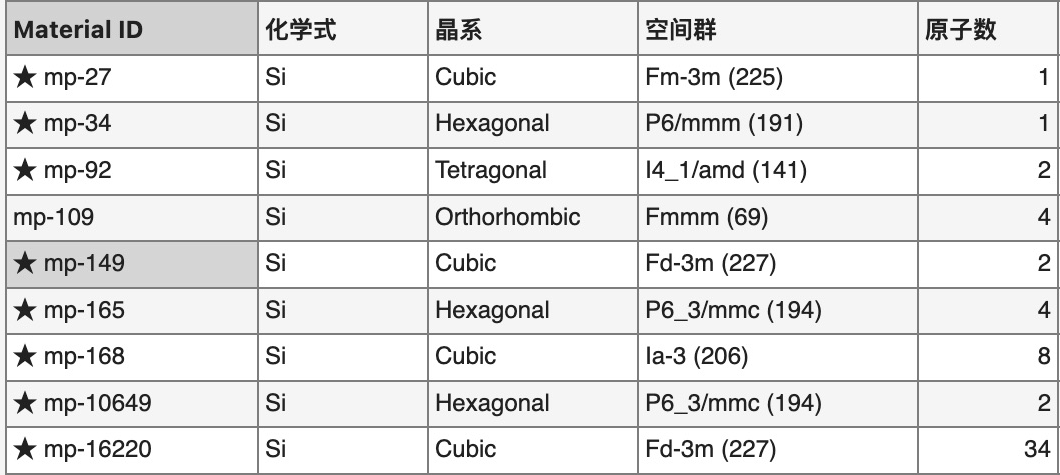
\includegraphics[width=\linewidth]{publication-assets/revision-materials-project-si-results-identity.png}
\caption{矽檢索結果的標識列區域性。此處選擇mp-149：Cubic、Fd-3m（227）、兩個原子；資料庫中還有其他矽晶型。}
\label{fig:mp-results-live}
\end{figure}

\begin{figure}[!htb]
\centering
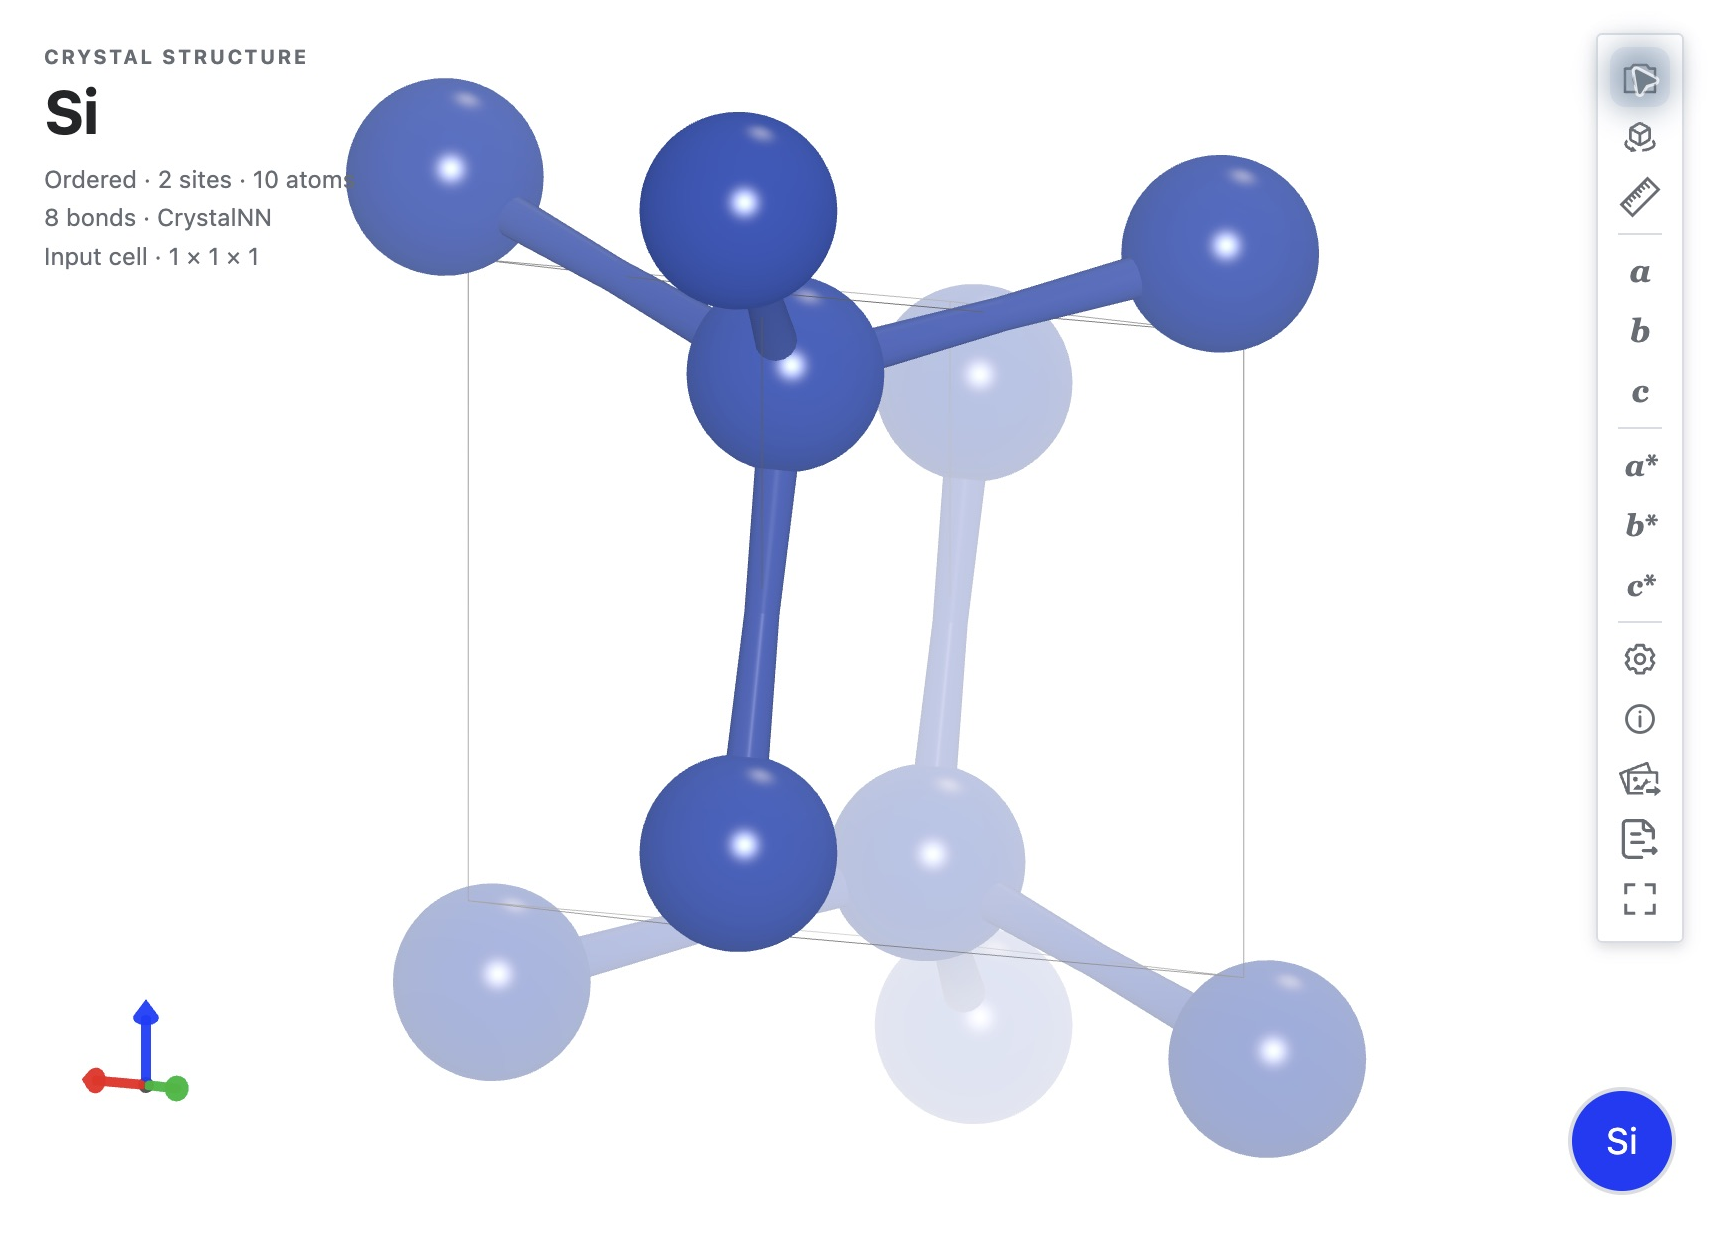
\includegraphics[width=\linewidth]{publication-assets/revision-materials-project-imported-si.png}
\caption{mp-149匯入後自動開啟的矽原胞檢視。摘要顯示兩個獨立位點，附加的半透明原子用於表示週期邊界連線。}
\label{fig:mp-import-live}
\end{figure}



\section{完成本章後的檢查}
現在應能在專案樹中找到匯入的矽結構，知道如何開啟和關閉文件，能夠收放側邊面板，並把工作儲存為 \file{.ks} 專案。繼續到第一項計算前，準備好隨書的氫分子案例，保留當前矽專案。後續章節還會使用矽作為示例，進行數值比較時按各章指定的結構檔案開始。
